%% 
%% Copyright 2007, 2008, 2009 Elsevier Ltd
%% 
%% This file is part of the 'Elsarticle Bundle'.
%% ---------------------------------------------
%% 
%% It may be distributed under the conditions of the LaTeX Project Public
%% License, either version 1.2 of this license or (at your option) any
%% later version.  The latest version of this license is in
%%    http://www.latex-project.org/lppl.txt
%% and version 1.2 or later is part of all distributions of LaTeX
%% version 1999/12/01 or later.
%% 
%% The list of all files belonging to the 'Elsarticle Bundle' is
%% given in the file `manifest.txt'.
%% 

%% Template article for Elsevier's document class `elsarticle'
%% with numbered style bibliographic references
%% SP 2008/03/01

\documentclass[preprint,12pt]{article}

\usepackage{graphicx} 	  %% The graphicx package provides the includegraphics command.
\usepackage{amssymb} 	%% The amssymb package provides various useful mathematical symbols

\usepackage{color}
\usepackage{amsmath}
\usepackage{mathtools}
\usepackage{fullpage}
\usepackage{algorithmic}
\DeclareMathOperator*{\argmin}{argmin}
\DeclareMathOperator*{\argmax}{argmax}
\algsetup{linenosize=\small}
\usepackage[table,xcdraw]{xcolor}
\usepackage{multirow}
\usepackage[super]{nth}
\usepackage{graphicx,adjustbox}
\usepackage{caption}
\usepackage[labelformat=simple]{subcaption}
\usepackage{comment}
\usepackage{setspace}
\usepackage{textcomp}
\usepackage{xspace}
\usepackage{siunitx}
\usepackage{epsfig}
\usepackage{epstopdf}
\usepackage{soul}
\usepackage{url}
\usepackage{tablefootnote}
\DeclareMathOperator{\E}{\mathbb{E}} % Expectation Symbol
\usepackage[linesnumbered,ruled]{algorithm2e}
\usepackage{booktabs}
\usepackage{hyperref}
\usepackage[normalem]{ulem}
\usepackage{footnote}
\usepackage[misc,geometry]{ifsym} 
\makesavenoteenv{tabular}

%% Other
\DeclarePairedDelimiter\abs{\lvert}{\rvert}

\renewcommand\thesubfigure{(\alph{subfigure})}
\let\OldTexttrademark\texttrademark
\renewcommand{\texttrademark}{\OldTexttrademark\xspace}%
\DeclarePairedDelimiter\ceil{\lceil}{\rceil}
%% Use the options 1p,twocolumn; 3p; 3p,twocolumn; 5p; or 5p,twocolumn
%% for a journal layout:
%% \documentclass[final,1p,times]{elsarticle}
%% \documentclass[final,1p,times,twocolumn]{elsarticle}
%% \documentclass[final,3p,times]{elsarticle}
%% \documentclass[final,3p,times,twocolumn]{elsarticle}
%% \documentclass[final,5p,times]{elsarticle}
%% \documentclass[final,5p,times,twocolumn]{elsarticle}

%\usepackage{authblk}

%% Use the option review to obtain double line spacing
%% \documentclass[authoryear,preprint,review,12pt]{elsarticle}

%% Use the options 1p,twocolumn; 3p; 3p,twocolumn; 5p; or 5p,twocolumn
%% for a journal layout:
%% \documentclass[final,1p,times]{elsarticle}
%% \documentclass[final,1p,times,twocolumn]{elsarticle}
%% \documentclass[final,3p,times]{elsarticle}
%% \documentclass[final,3p,times,twocolumn]{elsarticle}
%% \documentclass[final,5p,times]{elsarticle}
%% \documentclass[final,5p,times,twocolumn]{elsarticle}

%% For including figures, graphicx.sty has been loaded in
%% elsarticle.cls. If you prefer to use the old commands
%% please give \usepackage{epsfig}
\usepackage{epsfig}
%% The amssymb package provides various useful mathematical symbols
\usepackage{amssymb}
%% The amsthm package provides extended theorem environments
%% \usepackage{amsthm}
\newcommand{\francesc}[1]{\textcolor{blue}{#1}}
\newcommand{\francesco}[1]{\textcolor{orange}{#1}}
%% The lineno packages adds line numbers. Start line numbering with
%% \begin{linenumbers}, end it with \end{linenumbers}. Or switch it on
%% for the whole article with \linenumbers.
%% \usepackage{lineno}
\title{Asynchronous vs Synchronous Selfish Learning}

\begin{document}
\maketitle

\section{Introduction}
In order to decrease the temporal variability experienced by WNs applying online learning, we propose the following mechanism:
\begin{itemize}
	\item WNs are synchronized, so that they act at specific intervals.
	\item In each iteration, only one WN is able to select an action. Of course, it can select the one that is currently using (exploitation).
	\item Every WN that remains "static" in a given iteration is considered to choose the last selected action.
\end{itemize}

Two important implications are derived from the abovementioned mechanism: \emph{i)} the action-selection strategy of the learning algorithms are modified, \emph{ii)} the adversarial setting changes, so that the performance of every chosen action is potentially evaluated in a larger set of situations. According to the latter, a higher level of valuable knowledge is more likely to be provided to each arm. However, depending on the learning algorithm used, there can be other implications.
 
\section{Results - Toy Scenario}

\subsection{$\varepsilon$-greedy}
\label{section:e-greedy}

Figure \ref{fig:e_greedy} shows several results regarding the application of $\varepsilon$-greedy in the toy scenario (1,000 iterations are considered), both for the fully decentralized and the synchronized approaches. As shown, the latter allows to experience a lower temporal throughput variability (\ref{fig:temporal_individual_tpt_EG} vs \ref{fig:temporal_individual_tpt_OEG}), since a lower number of actions is being exploited (\ref{fig:actions_probability_EG} vs \ref{fig:actions_probability_OEG}). However, similar results are obtained with respect to the average throughput experienced per WN (\ref{fig:mean_tpt_EG} vs \ref{fig:mean_tpt_OEG}). The fact is that, for the synchronized approach, WNs tend to exploit sub-optimal actions for longer periods (while they wait for their turn). In contrast, WNs are able to rapidly discard these sub-optimal actions in their turn.

\begin{figure*}[h!]
	\centering
	\begin{subfigure}[b]{.3\textwidth}
		\includegraphics[width=\textwidth]{images/actions_probability_EG}
		\caption{Actions prob. (default)}\label{fig:actions_probability_EG}
	\end{subfigure}
	\begin{subfigure}[b]{.3\textwidth}
		\includegraphics[width=\textwidth]{images/actions_probability_OEG}
		\caption{Actions prob. (sync.)}\label{fig:actions_probability_OEG}
	\end{subfigure}
	\begin{subfigure}[b]{.3\textwidth}
		\includegraphics[width=\textwidth]{images/actions_probability_CEG}
		\caption{Actions prob. (sync. 2)}\label{fig:actions_probability_CEG}
	\end{subfigure}\\
	\begin{subfigure}[b]{.3\textwidth}
		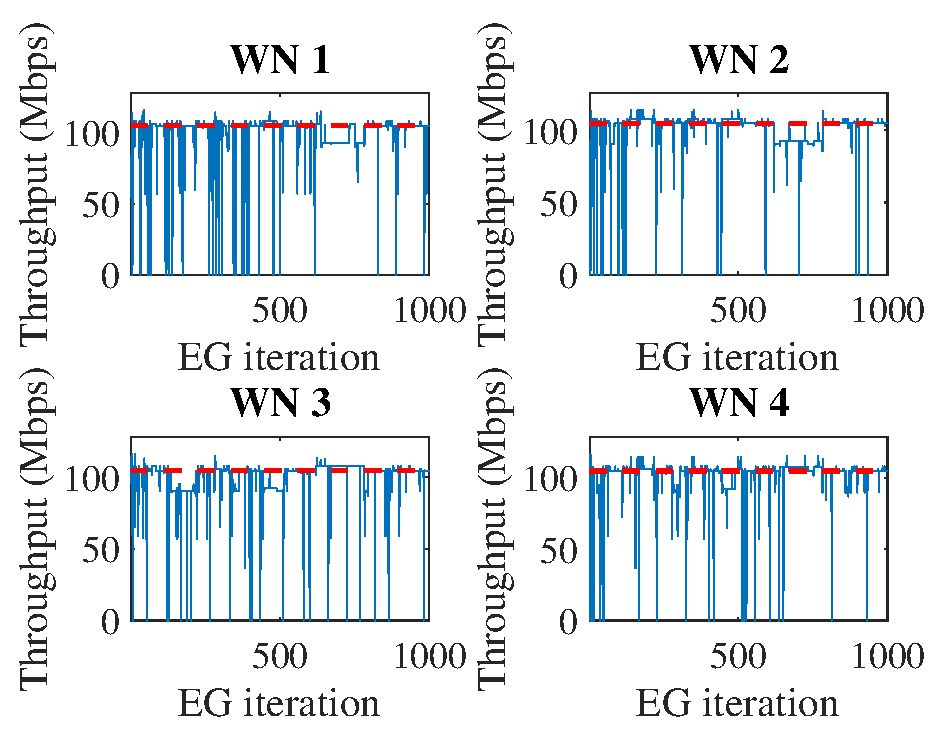
\includegraphics[width=\textwidth]{images/temporal_individual_tpt_EG}
		\caption{Temp. var.  (default)}\label{fig:temporal_individual_tpt_EG}
	\end{subfigure}
	\begin{subfigure}[b]{.3\textwidth}
		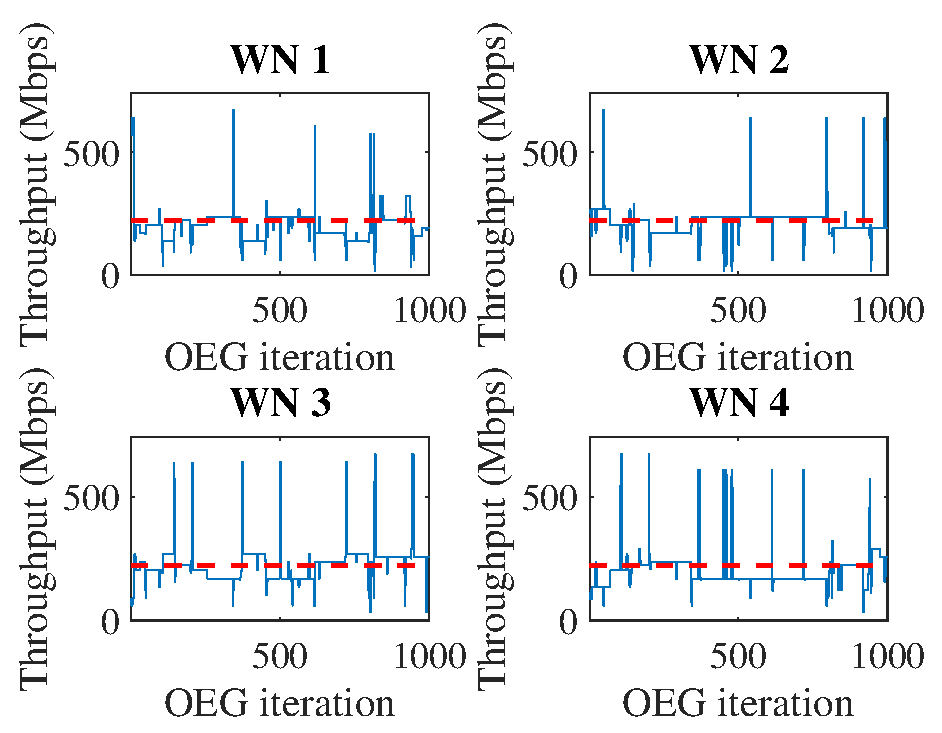
\includegraphics[width=\textwidth]{images/temporal_individual_tpt_OEG}
		\caption{Temp. var.  (sync.)}\label{fig:temporal_individual_tpt_OEG}
	\end{subfigure}
	\begin{subfigure}[b]{.3\textwidth}
		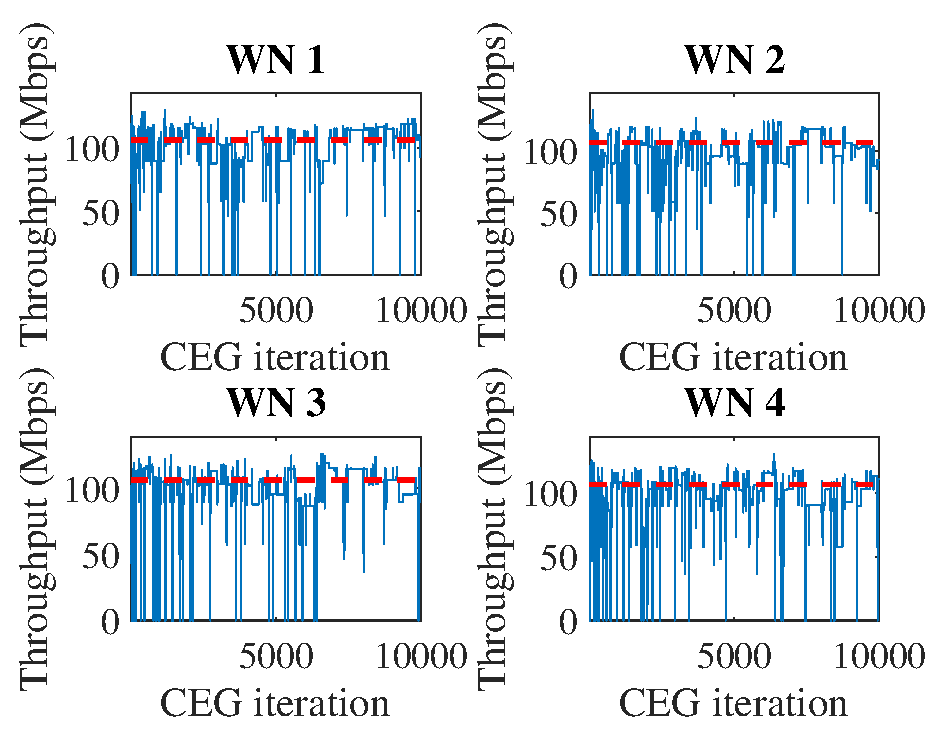
\includegraphics[width=\textwidth]{images/temporal_individual_tpt_CEG}
		\caption{Temp. var.  (sync. 2)}\label{fig:temporal_individual_tpt_CEG}
	\end{subfigure}\\
	\begin{subfigure}[b]{.3\textwidth}
		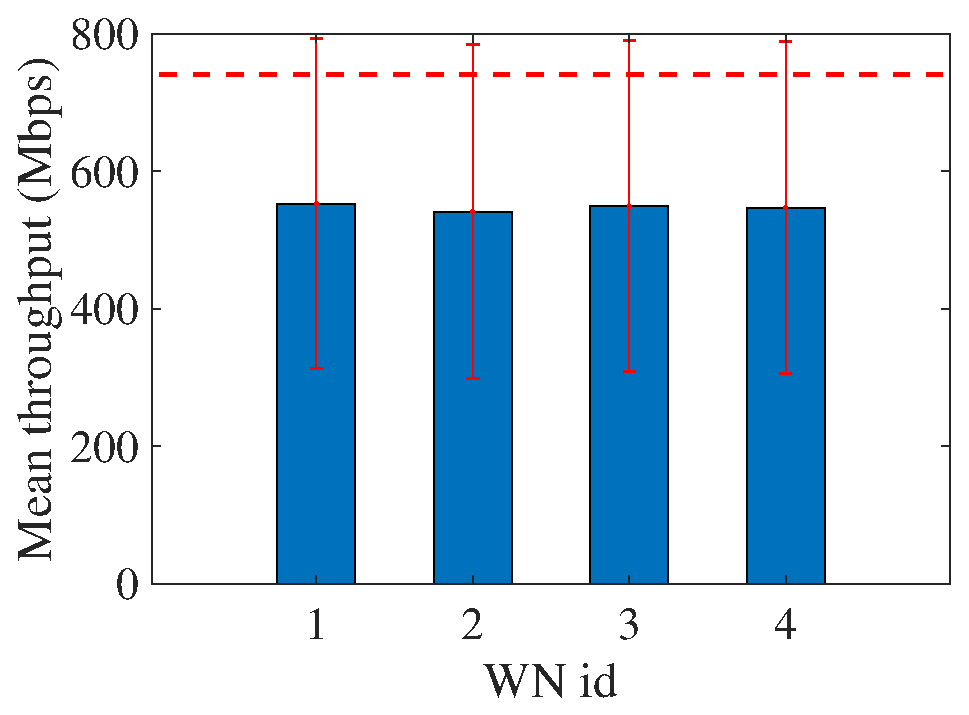
\includegraphics[width=\textwidth]{images/mean_tpt_EG}
		\caption{Mean tpt. (default)}\label{fig:mean_tpt_EG}
	\end{subfigure}
	\begin{subfigure}[b]{.3\textwidth}
		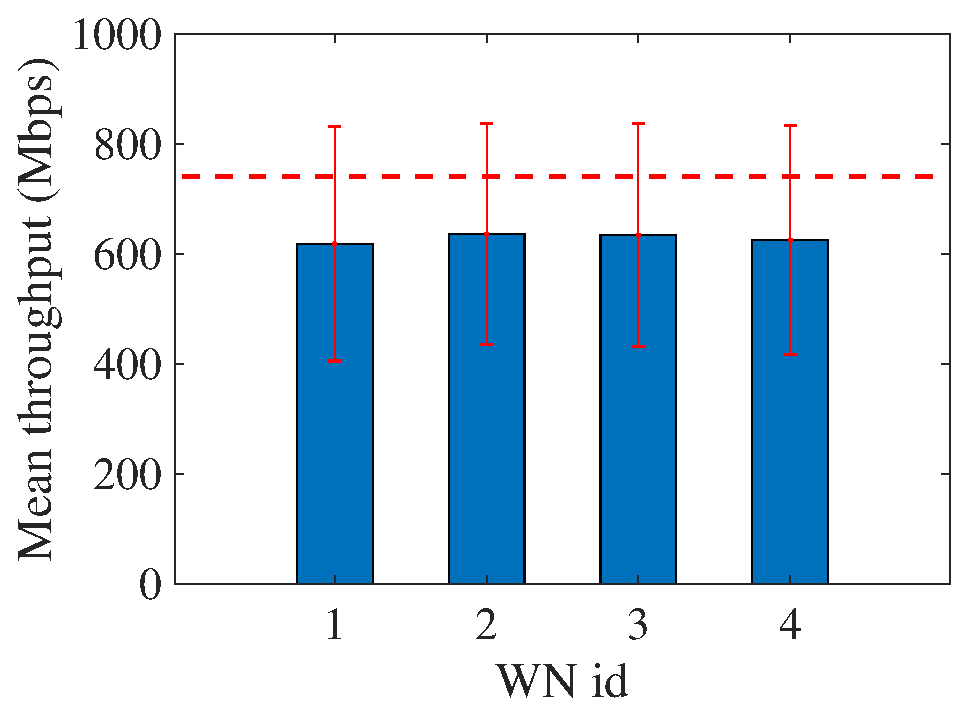
\includegraphics[width=\textwidth]{images/mean_tpt_OEG}
		\caption{Mean tpt. (sync.)}\label{fig:mean_tpt_OEG}
	\end{subfigure}
	\begin{subfigure}[b]{.3\textwidth}
		\includegraphics[width=\textwidth]{images/mean_tpt_CEG}
		\caption{Mean tpt. (sync. 2)}\label{fig:mean_tpt_CEG}
	\end{subfigure}
	\caption{Simulation results in $\varepsilon$-greedy (1,000 iterations)}
	\label{fig:e_greedy}
\end{figure*}

\subsection{EXP3}
\label{section:exp3}

Figure \ref{fig:exp3} shows several results regarding the application of EXP3 in the toy scenario (1,000 iterations are considered), both for the fully decentralized and the synchronized approaches. Again, the synchronized version of EXP3 leads to a lower temporal variability (\ref{fig:temporal_individual_tpt_EXP3} vs \ref{fig:temporal_individual_tpt_OEXP3}). No significant conclusions can be drawn for the actions probability profile (\ref{fig:actions_probability_EXP3} vs \ref{fig:actions_probability_OEXP3}), since in EXP3 it appears to be slightly random (recall that different EXP3 simulations may lead to different results). Finally, regarding the average throughput experienced per WN, similar "pseudo-randomized" results are obtained (\ref{fig:mean_tpt_EXP3} vs \ref{fig:mean_tpt_OEXP3}). 

\begin{figure*}[h!]
	\centering
	\begin{subfigure}[b]{.3\textwidth}
		\includegraphics[width=\textwidth]{images/actions_probability_EXP3}
		\caption{Actions prob. (default)}\label{fig:actions_probability_EXP3}
	\end{subfigure}
	\begin{subfigure}[b]{.3\textwidth}
		\includegraphics[width=\textwidth]{images/actions_probability_OEXP3}
		\caption{Actions prob. (sync.)}\label{fig:actions_probability_OEXP3}
	\end{subfigure}
	\begin{subfigure}[b]{.3\textwidth}
		\includegraphics[width=\textwidth]{images/actions_probability_CEXP3}
		\caption{Actions prob. (sync. 2)}\label{fig:actions_probability_CEXP3}
	\end{subfigure}\\
	\begin{subfigure}[b]{.3\textwidth}
		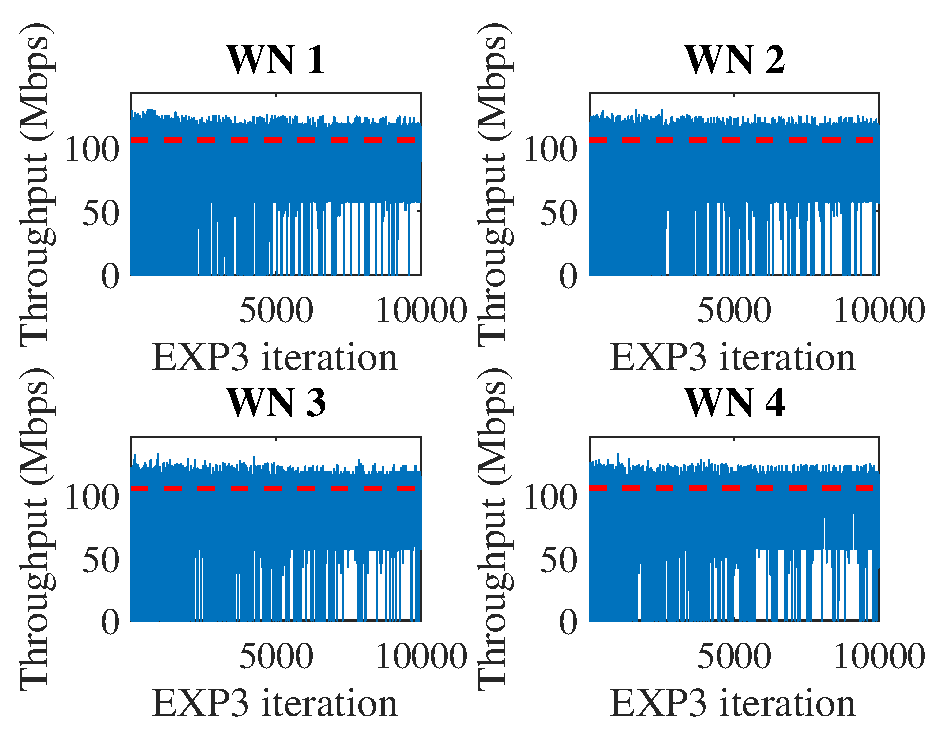
\includegraphics[width=\textwidth]{images/temporal_individual_tpt_EXP3}
		\caption{Temp. var.  (default)}\label{fig:temporal_individual_tpt_EXP3}
	\end{subfigure}
	\begin{subfigure}[b]{.3\textwidth}
		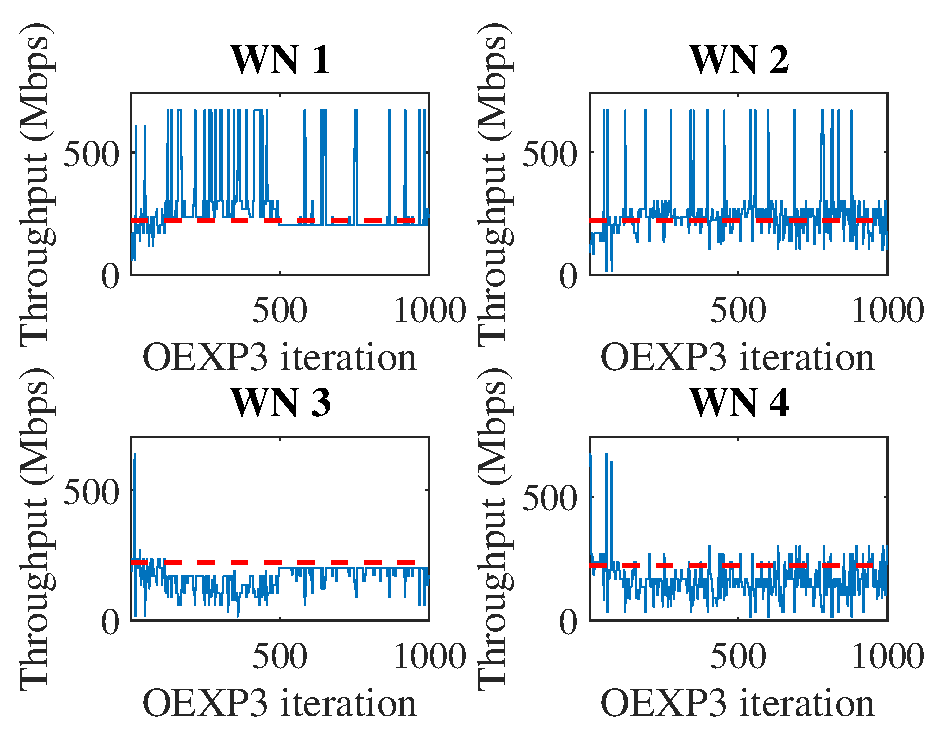
\includegraphics[width=\textwidth]{images/temporal_individual_tpt_OEXP3}
		\caption{Temp. var.  (sync.)}\label{fig:temporal_individual_tpt_OEXP3}
	\end{subfigure}
	\begin{subfigure}[b]{.3\textwidth}
		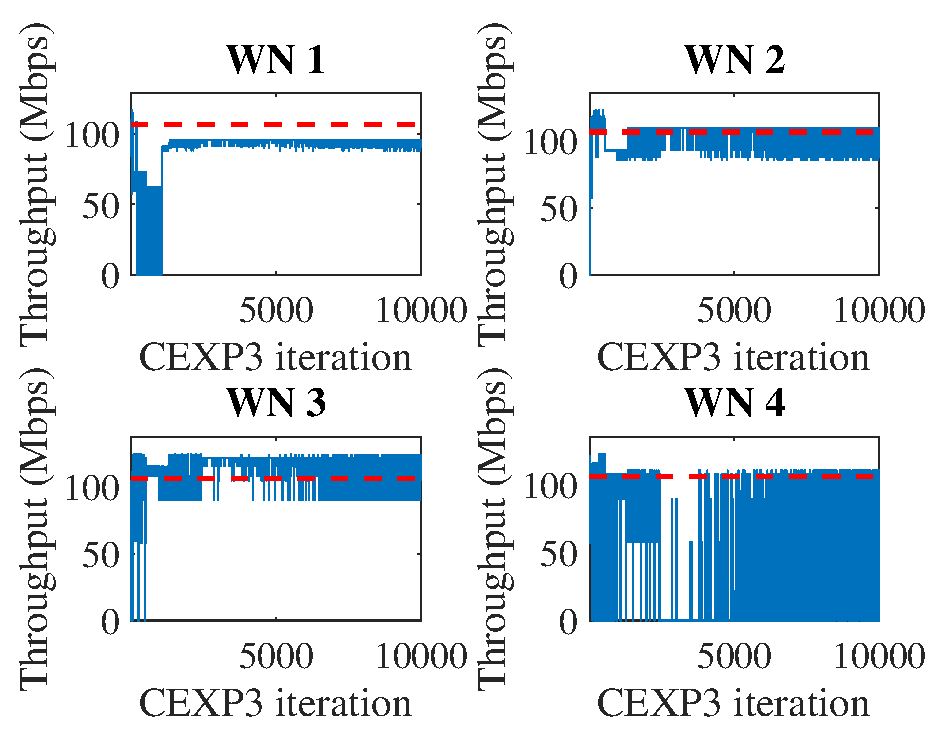
\includegraphics[width=\textwidth]{images/temporal_individual_tpt_CEXP3}
		\caption{Temp. var.  (sync.  2)}\label{fig:temporal_individual_tpt_CEXP3}
	\end{subfigure}\\
	\begin{subfigure}[b]{.3\textwidth}
		\includegraphics[width=\textwidth]{images/mean_tpt_EXP3}
		\caption{Mean tpt. (default)}\label{fig:mean_tpt_EXP3}
	\end{subfigure}
	\begin{subfigure}[b]{.3\textwidth}
		\includegraphics[width=\textwidth]{images/mean_tpt_OEXP3}
		\caption{Mean tpt. (sync.)}\label{fig:mean_tpt_OEXP3}
	\end{subfigure}
	\begin{subfigure}[b]{.3\textwidth}
		\includegraphics[width=\textwidth]{images/mean_tpt_CEXP3}
		\caption{Mean tpt. (sync. 2)}\label{fig:mean_tpt_CEXP3}
	\end{subfigure}
	\caption{Simulation results in EXP3 (1,000 iterations)}
	\label{fig:exp3}
\end{figure*}

\subsection{UCB}
\label{section:ucb}

Figure \ref{fig:ucb} shows several results regarding the application of UCB in the toy scenario (1,000 iterations are considered), both for the fully decentralized and the synchronized approaches. Unlike the previous cases, applying the synchronized approach to UCB is counter-productive, since its operational mode is altered by forcing WNs to choose undesired actions. As a result, the action-selection strategy is somehow randomized.

\begin{figure*}[h!]
	\centering
	\begin{subfigure}[b]{.3\textwidth}
		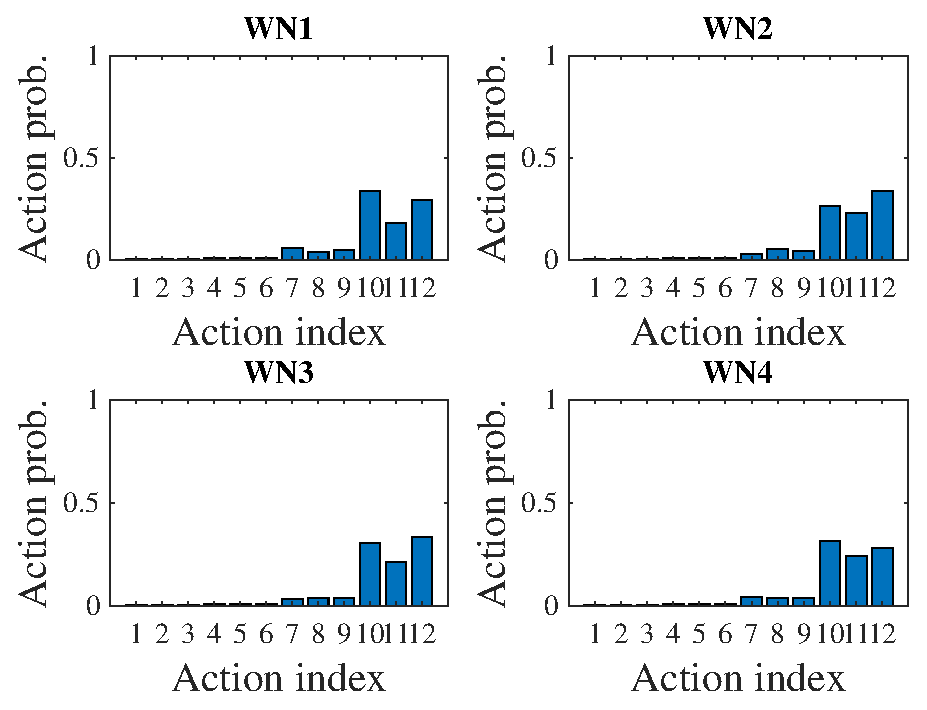
\includegraphics[width=\textwidth]{images/actions_probability_UCB}
		\caption{Actions prob. (default)}\label{fig:actions_probability_UCB}
	\end{subfigure}
	\begin{subfigure}[b]{.3\textwidth}
		\includegraphics[width=\textwidth]{images/actions_probability_OUCB}
		\caption{Actions prob. (sync.)}\label{fig:actions_probability_OUCB}
	\end{subfigure}
	\begin{subfigure}[b]{.3\textwidth}
		\includegraphics[width=\textwidth]{images/actions_probability_CUCB}
		\caption{Actions prob. (sync. 2)}\label{fig:actions_probability_CUCB}
	\end{subfigure}\\
	\begin{subfigure}[b]{.3\textwidth}
		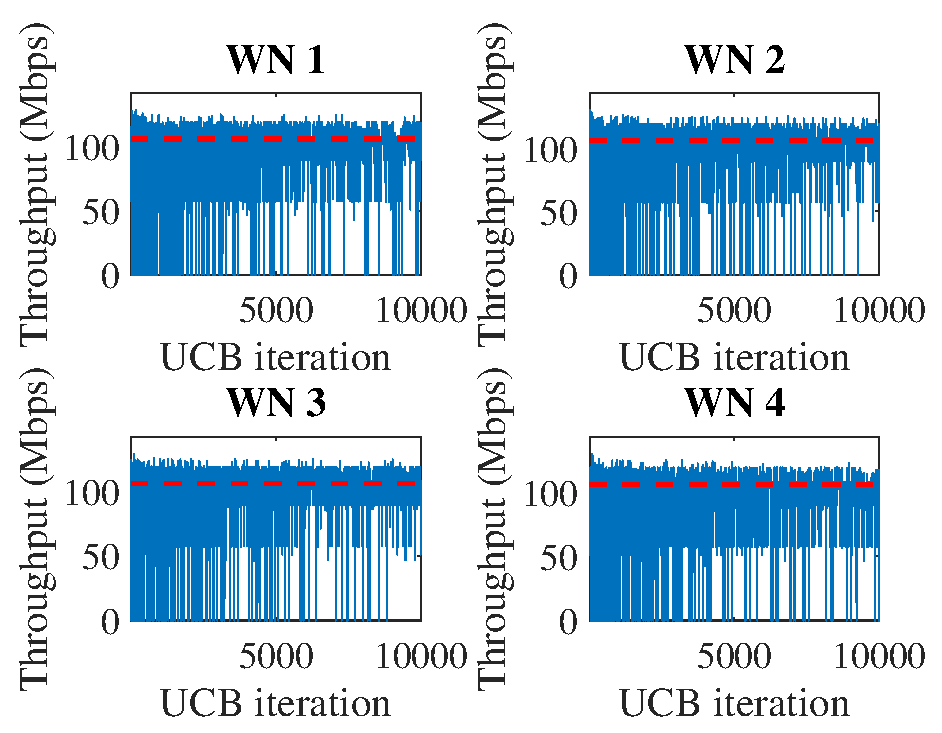
\includegraphics[width=\textwidth]{images/temporal_individual_tpt_UCB}
		\caption{Temp. var.  (default)}\label{fig:temporal_individual_tpt_UCB}
	\end{subfigure}
	\begin{subfigure}[b]{.3\textwidth}
		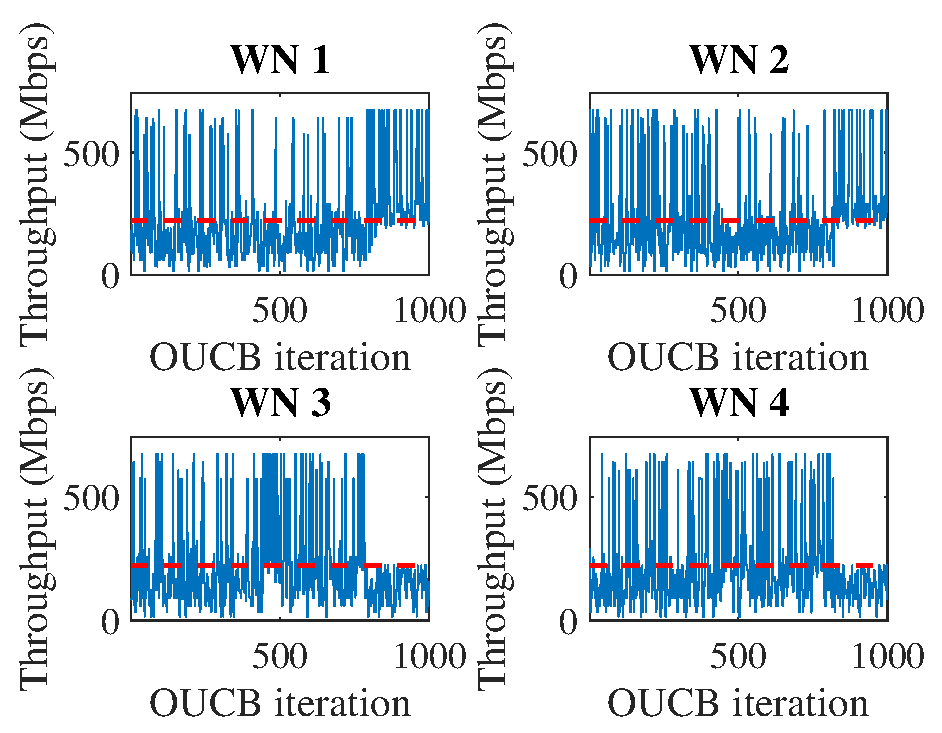
\includegraphics[width=\textwidth]{images/temporal_individual_tpt_OUCB}
		\caption{Temp. var.  (sync.)}\label{fig:temporal_individual_tpt_OUCB}
	\end{subfigure}
		\begin{subfigure}[b]{.3\textwidth}
		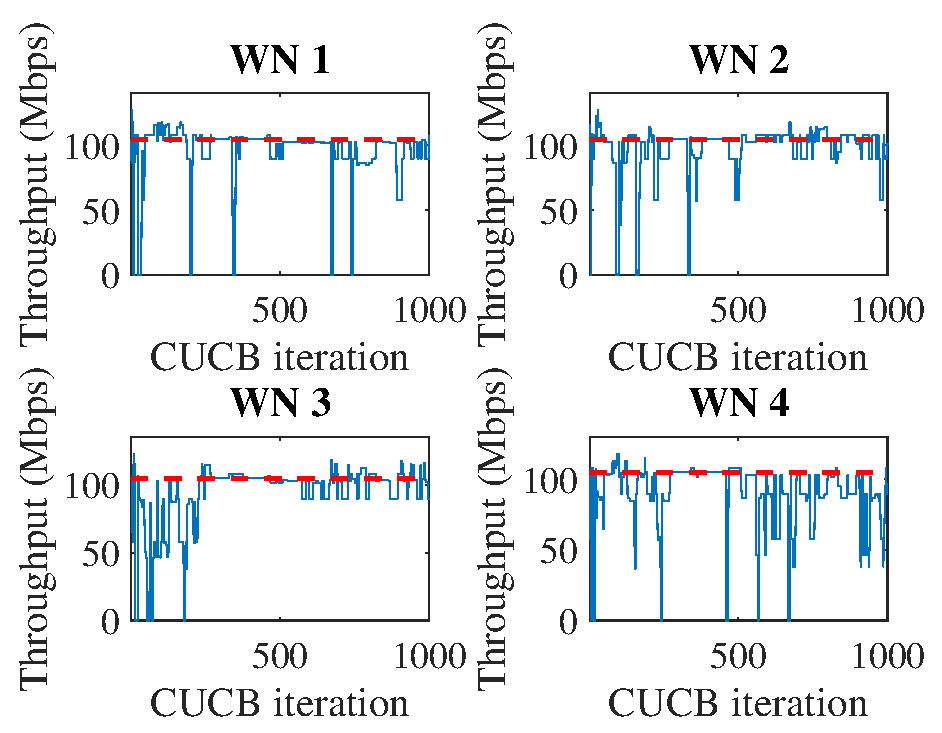
\includegraphics[width=\textwidth]{images/temporal_individual_tpt_CUCB}
		\caption{Temp. var.  (sync. 2)}\label{fig:temporal_individual_tpt_CUCB}
	\end{subfigure}\\
	\begin{subfigure}[b]{.3\textwidth}
		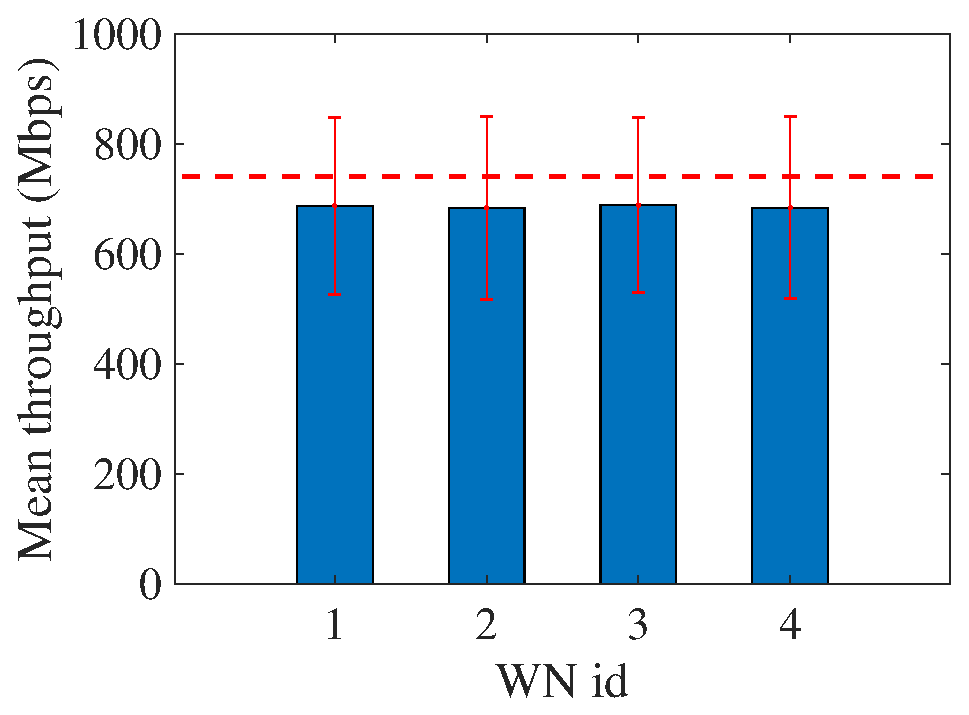
\includegraphics[width=\textwidth]{images/mean_tpt_UCB}
		\caption{Mean tpt. (default)}\label{fig:mean_tpt_UCB}
	\end{subfigure}
	\begin{subfigure}[b]{.3\textwidth}
		\includegraphics[width=\textwidth]{images/mean_tpt_OUCB}
		\caption{Mean tpt. (sync.)}\label{fig:mean_tpt_OUCB}
	\end{subfigure}
	\begin{subfigure}[b]{.3\textwidth}
		\includegraphics[width=\textwidth]{images/mean_tpt_CUCB}
		\caption{Mean tpt. (sync. 2)}\label{fig:mean_tpt_CUCB}
	\end{subfigure}
	\caption{Simulation results in UCB (1,000 iterations)}
	\label{fig:ucb}
\end{figure*}

\subsection{Thompson sampling}
\label{section:ts}

Figure \ref{fig:ts} shows several results regarding the application of Thompson sampling in the toy scenario (1,000 iterations are considered), both for the fully decentralized and the synchronized approaches. In this case, the temporal variability is significantly decreased (\ref{fig:temporal_individual_tpt_TS} vs \ref{fig:temporal_individual_tpt_OTS}). In contrast, the actions probability changes for the synchronized approach. In this case, some WNs (2 and 3) alternate two between actions. As it can be inferred from the temporal variability, one of the actions (the one granting lower performance) is selected until iteration 600 (approximately). At that moment, the best performing action (with respect to the adversarial environment) is chosen. This phenomena allegedly occurs when near-to-optimal actions are forced to be selected several times during the "static" periods. As a result, the algorithm provides high estimates to that actions, which are hard to be overtaken by the actual best-performing ones.

\begin{figure*}[h!]
	\centering
	\begin{subfigure}[b]{.3\textwidth}
		\includegraphics[width=\textwidth]{images/actions_probability_TS}
		\caption{Actions prob. (default)}\label{fig:actions_probability_TS}
	\end{subfigure}
	\begin{subfigure}[b]{.3\textwidth}
		\includegraphics[width=\textwidth]{images/actions_probability_OTS}
		\caption{Actions prob. (sync.)}\label{fig:actions_probability_OTS}
	\end{subfigure}
	\begin{subfigure}[b]{.3\textwidth}
		\includegraphics[width=\textwidth]{images/actions_probability_CTS}
		\caption{Actions prob. (sync. 2)}\label{fig:actions_probability_CTS}
	\end{subfigure}\\
	\begin{subfigure}[b]{.3\textwidth}
		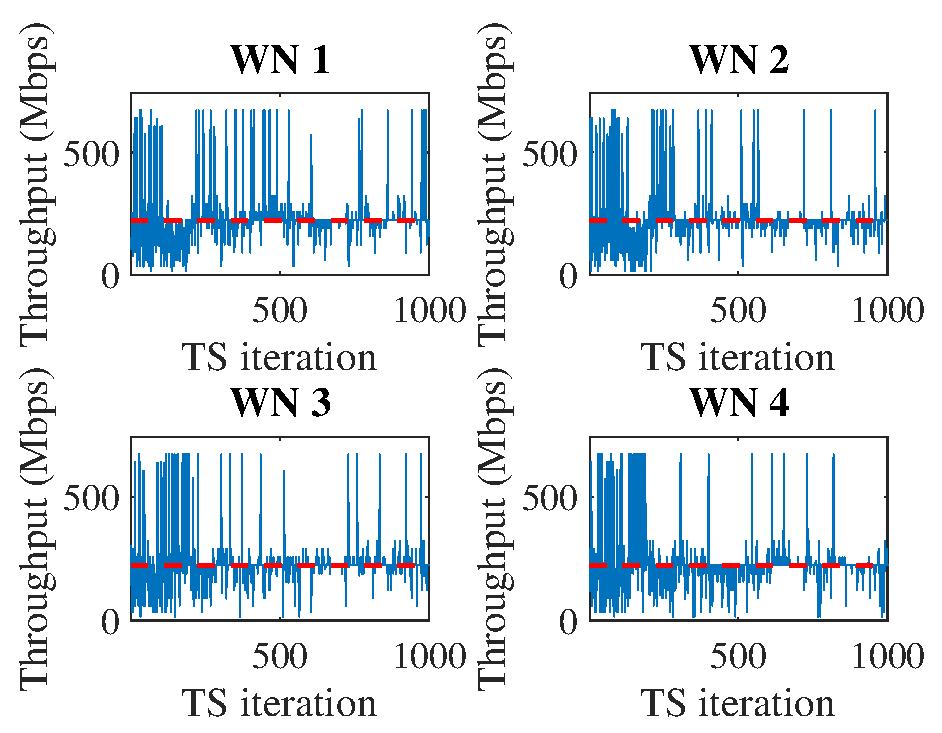
\includegraphics[width=\textwidth]{images/temporal_individual_tpt_TS}
		\caption{Temp. var.  (default)}\label{fig:temporal_individual_tpt_TS}
	\end{subfigure}
	\begin{subfigure}[b]{.3\textwidth}
		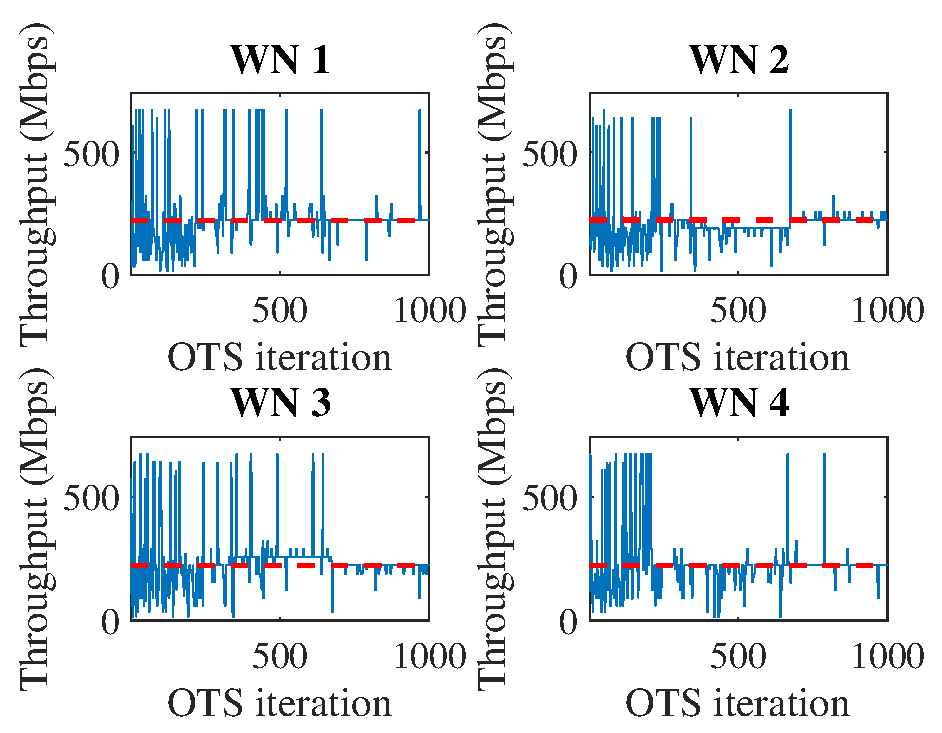
\includegraphics[width=\textwidth]{images/temporal_individual_tpt_OTS}
		\caption{Temp. var.  (sync.)}\label{fig:temporal_individual_tpt_OTS}
	\end{subfigure}
	\begin{subfigure}[b]{.3\textwidth}
		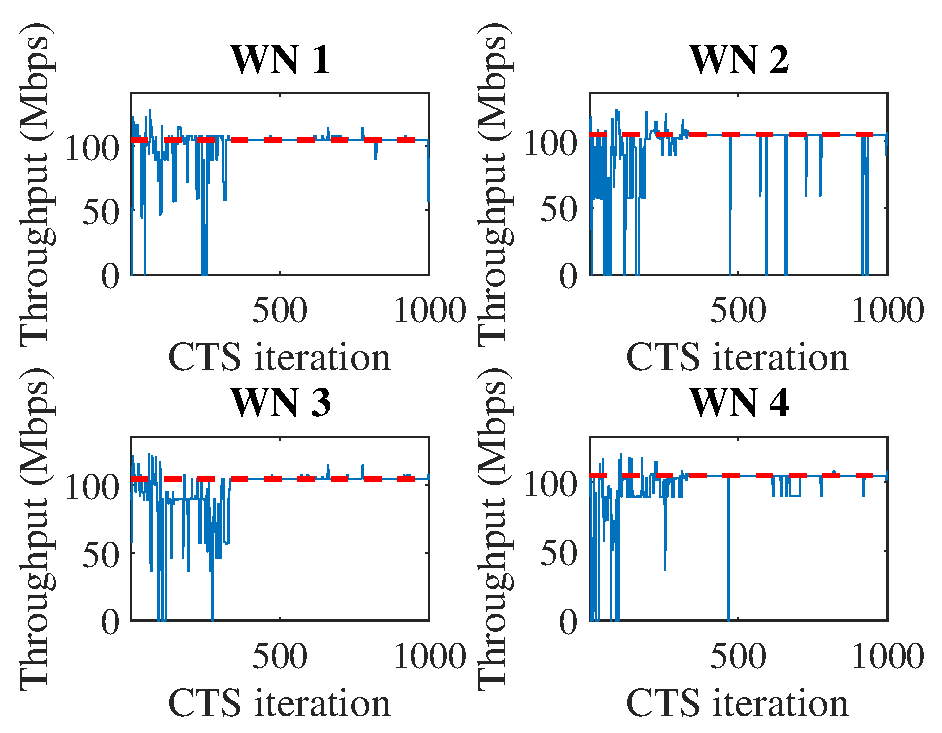
\includegraphics[width=\textwidth]{images/temporal_individual_tpt_CTS}
		\caption{Temp. var.  (sync. 2)}\label{fig:temporal_individual_tpt_CTS}
	\end{subfigure}\\
	\begin{subfigure}[b]{.3\textwidth}
		\includegraphics[width=\textwidth]{images/mean_tpt_TS}
		\caption{Mean tpt. (default)}\label{fig:mean_tpt_TS}
	\end{subfigure}
	\begin{subfigure}[b]{.3\textwidth}
		\includegraphics[width=\textwidth]{images/mean_tpt_OTS}
		\caption{Mean tpt. (sync.)}\label{fig:mean_tpt_OTS}
	\end{subfigure}
	\begin{subfigure}[b]{.3\textwidth}
		\includegraphics[width=\textwidth]{images/mean_tpt_CTS}
		\caption{Mean tpt. (sync. 2)}\label{fig:mean_tpt_CTS}
	\end{subfigure}
	\caption{Simulation results in Thompson sampling (1,000 iterations)}
	\label{fig:ts}
\end{figure*}

\section{Learning with penalties}
One promising possibility is to explore the effect of applying penalties to the reward, based on the transmit power or the saturation of a given channel (for that, we must know the number of users in each channel). Such penalties are not trivial to be derived, and when the problem becomes non-convex, the complexity increases. For that, we can provide some evidences about their usefulness when applying pure decentralized learning, but left its proper analysis as future work.

Here are some results for e-greedy when applying a penalty ($\alpha = 0.1$) to the transmit power used. The reward is now computed as:
\begin{equation}
	R = \frac{\Gamma}{\Gamma^*} - \alpha (\frac{TxPower}{max(TxPower)})
\end{equation}

As shown, WNs focus on few actions, which grant highest performance by considering the trade-off between the throughput and the power transmitted.

\begin{figure*}[h!]
	\centering
	\begin{subfigure}[b]{.3\textwidth}
		\includegraphics[width=\textwidth]{images/actions_probability_PEG}
		\caption{Actions prob. (penalty)}\label{fig:actions_probability_PEG}
	\end{subfigure}	
	\begin{subfigure}[b]{.3\textwidth}
		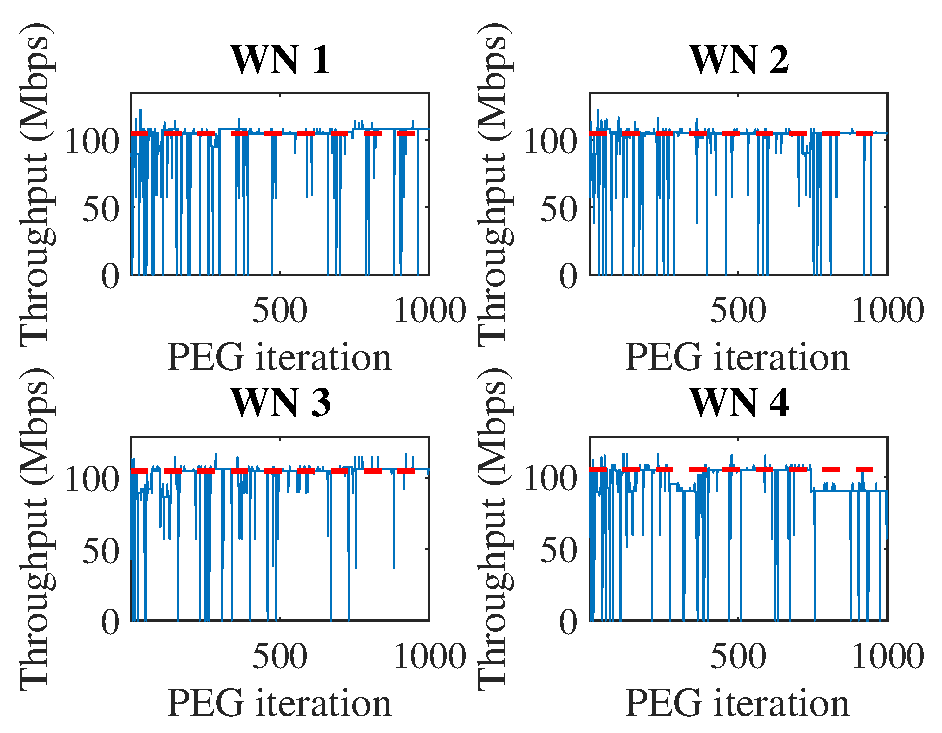
\includegraphics[width=\textwidth]{images/temporal_individual_tpt_PEG}
		\caption{Temp. var.  (penalty)}\label{fig:temporal_individual_tpt_PEG}
	\end{subfigure}
	\begin{subfigure}[b]{.3\textwidth}
		\includegraphics[width=\textwidth]{images/mean_tpt_PEG}
		\caption{Mean tpt. (penalty)}\label{fig:mean_tpt_PEG}
	\end{subfigure}
	\caption{Simulation results in Thompson sampling (1,000 iterations)}
	\label{fig:ts}
\end{figure*}

%\section{Results - Random Scenario}
%In order to reduce the simulation time, we have considered 1,000 learning iterations, rather than 10,000. In order to further illustrate the effect of applying synchronized selfish learning, we compare it with the default decentralized approach in the random scenarios. In this case, we use the realistic range of actions in both situations. As shown in Figure \ref{fig:scalability_sync_vs_async}, the synchronized mechanisms lead to less variability than their default versions (the histogram tends to be narrower for all the cases). In contrast, some performance loss can be observed, especially for the UCB algorithm (note that the blue distribution is slightly shifted to the left, with respect to the red one). 
%
%\begin{figure*}[h!]
%	\centering
%	\begin{subfigure}[b]{.4\textwidth}
%		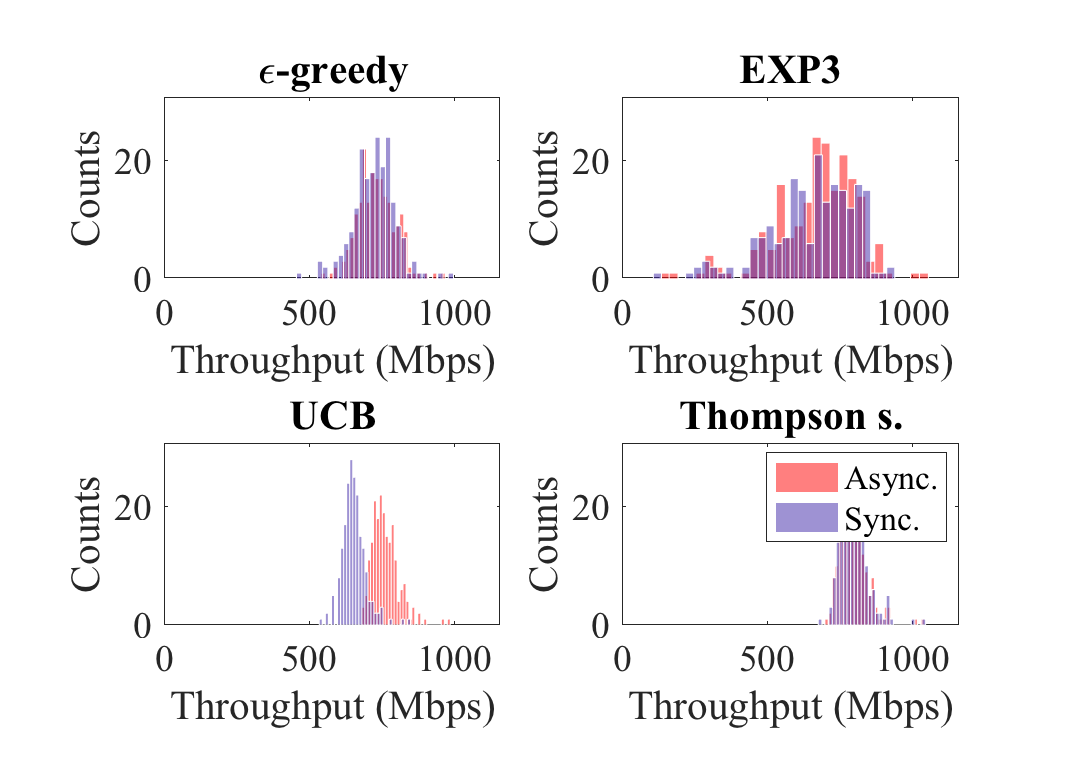
\includegraphics[width=\textwidth]{images/hist_mean_tpt_2_WNs}
%		\caption{2 WNs}\label{fig:hist_mean_tpt_2_WNs}
%	\end{subfigure}
%	\begin{subfigure}[b]{.4\textwidth}
%		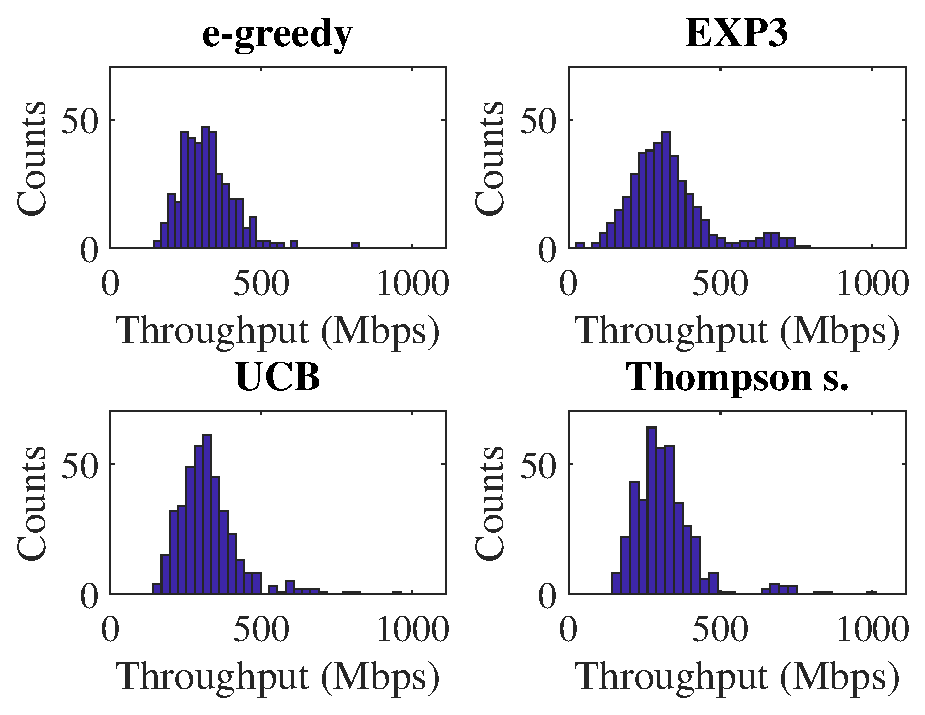
\includegraphics[width=\textwidth]{images/hist_mean_tpt_4_WNs}
%		\caption{4 WNs}\label{fig:hist_mean_tpt_4_WNs}
%	\end{subfigure}\\
%	\begin{subfigure}[b]{.4\textwidth}
%		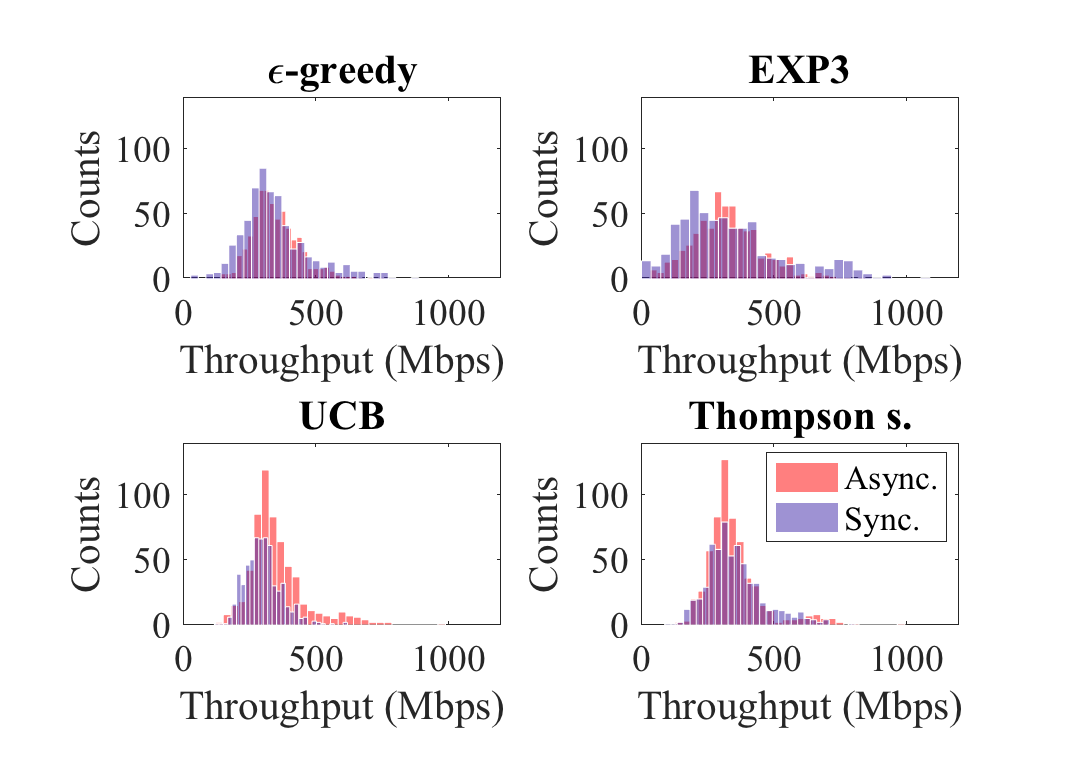
\includegraphics[width=\textwidth]{images/hist_mean_tpt_6_WNs}
%		\caption{6 WNs}\label{fig:hist_mean_tpt_6_WNs}
%	\end{subfigure}
%	\begin{subfigure}[b]{.4\textwidth}
%		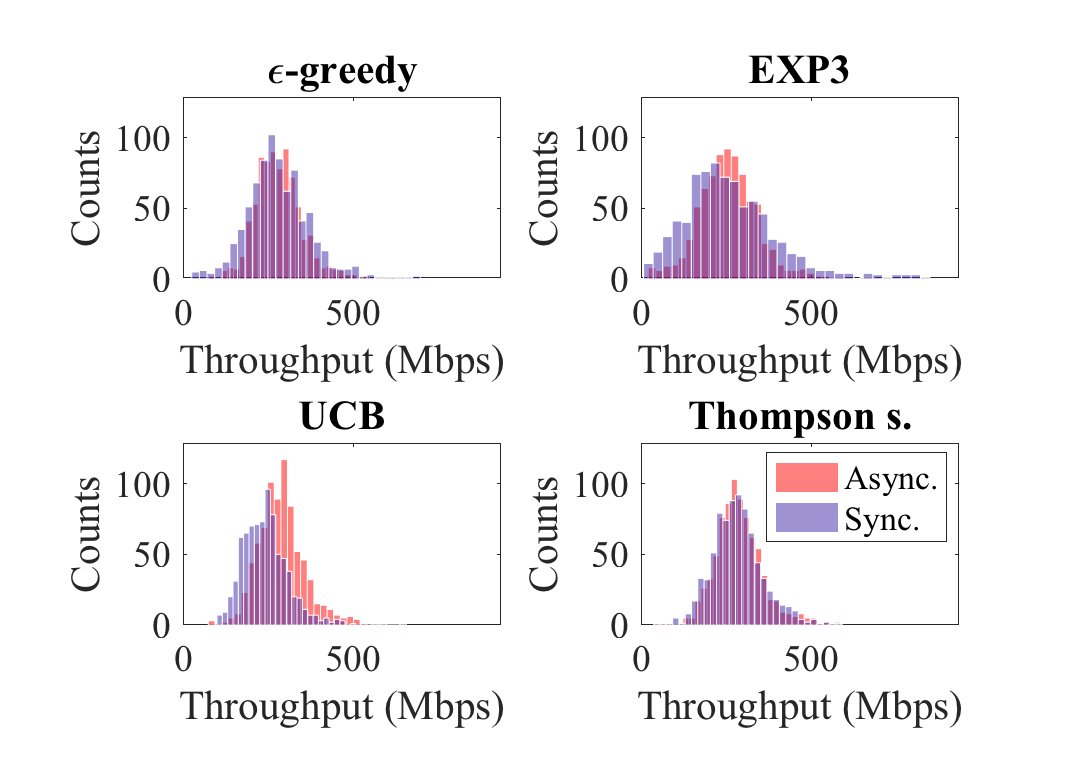
\includegraphics[width=\textwidth]{images/hist_mean_tpt_8_WNs}
%		\caption{8 WNs}\label{fig:hist_mean_tpt_8_WNs}
%	\end{subfigure}
%	\caption{Histogram of the mean throughput experienced by WNs for each algorithm. The results are computed from 100 different random scenarios for each of the WNs sizes, where 1,000 learning iterations are considered. In red, we have the results for the default algorithms implementation, while blue indicates their synchronized versions.}
%	\label{fig:scalability_sync_vs_async}
%\end{figure*}
%
%\section{Impact of modifying the range of actions}
%Here we aim to measure the impact of modifying the range of actions on the performance of the learning algorithms. For that, for each of the proposed action-selection strategies, we will compare the following performance measurements in the grid scenario, for different number of available actions: \emph{i)} the mean throughput experienced in average, \emph{ii)} the mean variability experienced in average.
%
%Firstly, Figures \ref{fig:impact_num_channels} and \ref{fig:impact_num_channels_on_variability} show the impact of using different number of orthogonal channels for each algorithm. As shown in \ref{fig:impact_num_channels}, the mean throughput increases until reaching 4 channels, so that each WN is able to properly access to a single channel. Such an ideal case is achieved by Thompson sampling and UCB. However, for $\varepsilon$-greedy and EXP3 we notice some performance anomalies when the number of available channels increases. Regarding the experienced variability (\ref{fig:impact_num_channels_on_variability}), we observe a peak when the number of channels is 3, situation in which at least two WNs are permanently in conflict, since they are competing for the same channel resources. Note that, for the other cases where the number of channels is not enough to accommodate all the WNs, a lower variability is experienced due to the impossibility of achieving a better performance.
%
%Secondly, the impact of modifying the available levels of transmit power is shown in both \ref{fig:impact_tx_power_levels_on_throughput} and \ref{fig:impact_tx_power_levels_on_variability}. In this case, we use the following sets of transmit power levels:
%\begin{itemize}
%	\item Set 1: \{5, 20\} dBm
%	\item Set 2: \{5, 10, 15, 20\} dBm
%	\item Set 3: from 2 to 20 dBm in steps of 2 dBm
%	\item Set 4: from 1 to 20 dBm in steps of 1 dBm
%\end{itemize}
%Regarding the throughput experienced (\ref{fig:impact_tx_power_levels_on_throughput}), we notice a very low variability when different sets of transmit power levels are used. In contrast, increasing the number of transmission power levels affects to the variability experienced by WNs. Such a variability increases in case of UCB and Thompson sampling. Different effects are noticed for $\varepsilon$-greedy and EXP3.
%
%\begin{figure*}[h!]
%	\centering
%	\begin{subfigure}[b]{.4\textwidth}
%		\includegraphics[width=\textwidth]{images/impact_num_channels}
%		\caption{Channel impact on the throughput}\label{fig:impact_num_channels}
%	\end{subfigure}
%	\begin{subfigure}[b]{.4\textwidth}
%		\includegraphics[width=\textwidth]{images/impact_num_channels_on_variability}
%		\caption{Channel impact on the variability}\label{fig:impact_num_channels_on_variability}
%	\end{subfigure}\\
%	\begin{subfigure}[b]{.4\textwidth}
%		\includegraphics[width=\textwidth]{images/impact_tx_power_levels_on_throughput}
%		\caption{TxPow impact on the throughput}\label{fig:impact_tx_power_levels_on_throughput}
%	\end{subfigure}
%	\begin{subfigure}[b]{.4\textwidth}
%		\includegraphics[width=\textwidth]{images/impact_tx_power_levels_on_variability}
%		\caption{TxPow impact on the variability}\label{fig:impact_tx_power_levels_on_variability}
%	\end{subfigure}
%	\caption{Mean and standard deviation of the throughput experienced in average when using different sets of actions.}
%	\label{fig:impact_actions}
%\end{figure*}

\end{document}